\chapter{Detectability in next-generation galaxy surveys}
\label{chapter:detect}

The Fourier galaxy bispectrum is complex, with the imaginary part arising from leading-order relativistic corrections, due to Doppler, gravitational redshift  and related line-of-sight effects  in redshift space. The detection of the imaginary  part of the bispectrum is potentially a smoking gun signal of relativistic contributions. Long-mode relativistic effects couple to  short-mode Newtonian effects in the galaxy bispectrum, but not in the galaxy power spectrum. This is  the basis for detectability of relativistic effects in the bispectrum of a single galaxy survey, whereas the power spectrum requires multiple galaxy surveys to detect the corresponding signal.

In this chapter, we investigate whether the next generation of high-precision cosmological surveys will be able to make such a detection. First, we consider a Stage IV spectroscopic $H\alpha$ survey similar to Euclid, and we find that the cumulative signal to noise of this relativistic signature  is $\ord(10)$. Secondly, we look at some future 21cm intensity mapping surveys; MeerKAT, SKA, PUMA, and HIRAX. Due to foreground and telescope beam effects, the signal-to-noise ratio for intensity mapping surveys is typically lower than for spectroscopic $H\alpha$ surveys, though also still detectable.

\section{Introduction}

The bispectrum of number count fluctuations in redshift space will become an increasingly important complement to the power spectrum in the extraction of cosmological information from galaxy surveys, 
{in the measurement of {clustering} bias parameters and in the breaking of degeneracies between the clustering amplitude and growth rate.}
Analysis of the Fourier galaxy bispectrum is already well advanced for existing survey data (e.g \cite{Gil-Marin:2016wya,Sugiyama:2018yzo}) and for mock data of future surveys (e.g. \cite{Karagiannis:2018jdt,Yankelevich:2018uaz,Oddo:2019run,Sugiyama:2019ike}).  

Here we highlight a feature of the tree-level Fourier galaxy bispectrum which follows from the  leading-order relativistic contribution -- due to Doppler, gravitational redshift  and related line-of-sight effects -- that is omitted in the standard Newtonian analysis. These effects generate an imaginary part of the galaxy bispectrum, which can be understood as follows (see also \cite{McDonald:2009dh,Clarkson:2018dwn,Jeong:2019igb} for a more general discussion).  
The Doppler-type contributions to the galaxy density contrast involve one or three derivatives  of scalars along the fixed line of sight $\bm n$ [see \eqref{dg1}, \eqref{eq:dgsecond} below]. In Fourier space, with the plane-parallel approximation, we have  $\bm{n}\cdot\bm{\nabla} \to {\i}\, \bm{n}\cdot\bm{k}$, and this leads to imaginary corrections to the galaxy density contrast, which do not cancel in the bispectrum, unlike in the power spectrum. At first order, we have $\delta_g=\delta_{g\mathrm{N}}+ \delta_{g\mathrm{D}}$, where the Newtonian part $\delta_{g\mathrm{N}}$ is real and scales as the linear matter density contrast $\delta$. The 
relativistic Doppler-type part $\delta_{g\mathrm{D}}$ scales as ${\i}\,(\cH/k) \delta$  (see \cite{McDonald:2009dh, Jeong:2011as, Abramo:2017xnp,Clarkson:2018dwn} and below). At second  order, the relativistic contribution $\delta_{g\mathrm{D}}^{(2)}$ scales as ${\i}\,(\cH/k) (\delta)^2$ (see \cite{Clarkson:2018dwn} and below). 


In the case of  the galaxy {auto}-power spectrum, $P_g\sim \langle |\delta_g|^2\rangle$, the relativistic part is {real and scales as} $(\cH/k)^2P$\,:  therefore we can neglect $P_{g\mathrm{D}}$ at leading order. By contrast, for the galaxy bispectrum, $B_g\sim \langle \delta_g\,\delta_g \, \delta^{(2)}_g\rangle$, a coupling of relativistic contributions to short-scale Newtonian terms (which  is absent in $P_g$) produces a $B_{g\mathrm{D}}$ that is {imaginary and scales as} ${\i}\,(\cH/k)P^2$. 
We therefore expect these relativistic effects to be more accessible in the bispectrum than in the power spectrum, for the case of a single tracer {of the matter distribution}. 

Although the galaxy bispectrum is statistically isotropic, the plane-parallel approximation in redshift space breaks 3-dimensional isotropy, since a preferred direction is imposed by the observer's fixed line of sight. 

Let us introduce a more explicit analysis, as follows.

At tree-level, the Fourier galaxy bispectrum at  a redshift $z$ is given by
\begin{equation}
{\big\langle \delta_g(z,\bm{k}_{1})\delta_g(z,\bm{k}_{2})\delta^{(2)}_g(z,\bm{k}_{3}) \big\rangle + \text{2 cp}=2 (2\pi)^3 B_{g}(z, \bm{k}_{1}, \bm{k}_{2}, \bm{k}_{3}) \delta^{\mathrm{Dirac}}\big(\bm{k}_{1}+ \bm{k}_{2}+ \bm{k}_{3} \big)\,,}
\end{equation}
where cp denotes cyclic permutation and the factor 2 on the right arises from the convention that the total number density contrast is $\delta_g+ \delta^{(2)}_g/2$.  
In terms of the first- and second-order kernels, we have
\begin{equation}
B_{g}(z, \bm{k}_{1}, \bm{k}_{2}, \bm{k}_{3}) = \mathcal{K}^{(1)}(z, \bm{k}_{1})\mathcal{K}^{(1)}(z, \bm{k}_{2})\mathcal{K}^{(2)}(z, \bm{k}_{1}, \bm{k}_{2}, \bm{k}_{3})P(z, k_{1})P(z, k_{2}) + \text{2 cp}\,, \label{eq:bkern}
\end{equation}
where $P$ is the linear matter power spectrum. 
The $9-3=6$ degrees of freedom in the triangle condition $\bm{k}_{1}+ \bm{k}_{2}+ \bm{k}_{3}=\bm{0}$ at each $z$ are reduced to 5 by the fixed observer's line of sight direction $\bm{n}$.
The bispectrum can be chosen at each $z$ to be a function  of the 3 magnitudes ${k_a}=\big({k}_{1}, {k}_{2},{k}_{3}\big)$ and 2 angles that define the orientation of the triangle (see Fig. \ref{fig0}):
\begin{equation}
B_{g}(z, \bm{k}_{a}) =B_{g}(z, {k}_{a},  \mu_1,\varphi) \,.
\end{equation}
Here $\mu_a=\hat{\bm{k}}_a\cdot\bm{n}=\cos\theta_a$,  and $\varphi$ is the angle between the triangle plane and the $(\bm{n},\bm{k}_1)$-plane. The three angles $\theta_{ab}= \cos^{-1}\big(\hat{\bm{k}}_{a} \cdot \hat{\bm{k}}_b\big)$, are determined by $k_a$; then $\mu_2=\mu_1\cos\theta_{12}+ \sin\theta_1\,\sin\theta_{12}\cos\varphi$ is determined when $\varphi$ is given, and $\mu_3=-(\mu_1k_1+\mu_2k_2)/k_3$.
\begin{figure}[ht]
\centering
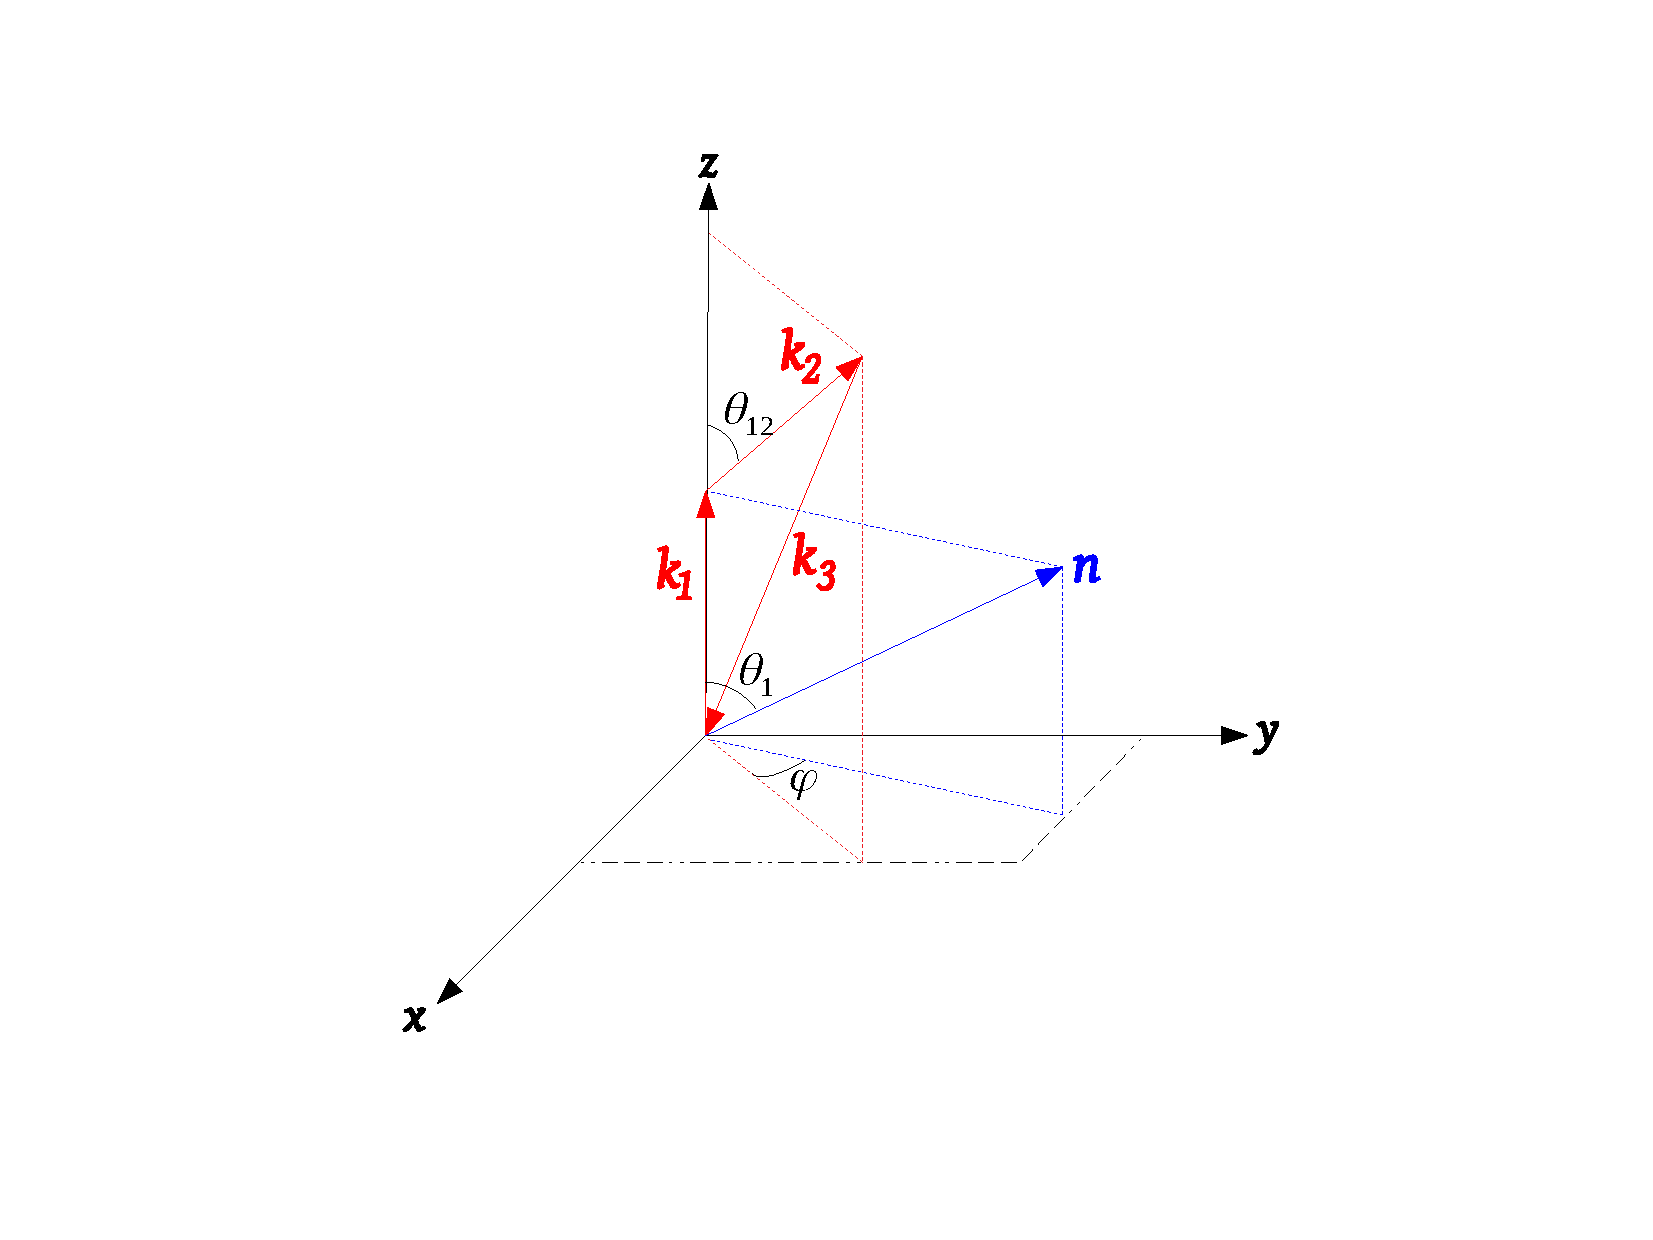
\includegraphics[width=10.0cm]{fig/geometryAngles}
\vspace*{-1cm}
\caption{Relevant vectors and angles for the Fourier bispectrum.} \label{fig0}
\end{figure}

In the standard Newtonian approximation, $B_g=B_{g{\mathrm{N}}}$, the kernels in \eqref{eq:bkern} contain the galaxy bias and the redshift-space distortions (RSD) at first and second order \cite{Bernardeau:2001qr, Karagiannis:2018jdt}:
\begin{align}
\mathcal{K}^{(1)}_{\mathrm{N}}(\bm{k}_{1}) &= b_{1}+f\mu_{1}^{2}\,,  \label{e15} \\ 
{\mathcal{K}^{(2)}_{\mathrm{N}}}(\bm{k}_{1}, \bm{k}_{2},{\bm{k}_3}) &= b_{1}F_{2}(\bm{k}_{1}, \bm{k}_{2}) + b_{2} + f\mu_{3}^{2}G_{2}(\bm{k}_{1}, \bm{k}_{2}) +{fZ_2}(\bm{k}_{1}, \bm{k}_{2})
+ b_{s^{2}}S_{2}(\bm{k}_{1}, \bm{k}_{2}) , \label{k2n}
\end{align}
where we dropped the $z$-dependence for brevity. Here $f$ is the linear matter growth rate, $b_1,b_2$ are the linear and second-order clustering biases, and $b_{s^{2}}$ is the tidal bias. The kernel  $F_2$ is for second-order density, $G_2 , \mathcal{Z}_2$ are for RSD,  and $S_2$  is the kernel for tidal bias (see Appendix~\ref{app_euclid} for the full expressions).


The Doppler-type relativistic corrections to the Newtonian number count contrast in redshift space are  given {at first order by \cite{Bonvin:2011bg}:}
\begin{equation}
\delta_{g\mathrm{D}} =  {A}\,\bm{v}\cdot\bm{n}\,,\label{dg1}
\end{equation}
{where $A(z)$ is given below in \eqref{e25} and the momentum conservation equation has been used to  eliminate the gravitational redshift: $\bm{n}\cdot\bm{\nabla}\Phi\equiv \p_r \Phi = -\bm{v}'\!\cdot\bm{n}-\cH\,\bm{v}\cdot\bm{n} $.} Here $\Phi$ is the gravitational potential, $\bm{v}$ is the peculiar velocity,  $\cH$ is the comoving Hubble parameter, and $r$ is the line-of-sight comoving distance.
Note that $\bm{v}\cdot\bm{n}=\partial_r V$, where $V$ is the velocity potential ($v_i=\partial_iV$). 
At second order, and neglecting vector and tensor modes, it is shown in
\cite{Clarkson:2018dwn}  that (see also \cite{DiDio:2018zmk}) 
\begin{align}
\delta^{(2)}_{g{\mathrm{D}}}&= A\, \bm{v}^{(2)}\!\!\cdot\bm{n}+2{C}(\bm{v}\cdot\bm{n})\,\delta +2 \frac{{E}}{\cH}(\bm{v}\cdot\bm{n})\,\partial_r(\bm{v}\cdot\bm{n})
+ \frac{2}{\cH^2}\big[(\bm{v}\cdot\bm{n}) \,\partial_r^2\Phi-\Phi\, \partial_r^2 (\bm{v}\cdot\bm{n}) \big]
\nonumber\\ \label{eq:dgsecond}
& - \frac{2}{\cH}\,\partial_r (\bm{v}\cdot\bm{v}) + 2 \frac{b_1}{\cH}\,\Phi\, \partial_r\delta \,. 
\end{align}
The redshift-dependent coefficients $C,E$ are  given below  in \eqref{e26}, \eqref{e27}.


In Fourier space, 
neglecting sub-leading $ \mathcal{O}(\cH^2/k^2)$ terms, we find from \eqref{eq:bkern} that
\begin{align}
 B_{g\mathrm{D}}(\bm{k}_{1},\bm{k}_{2},\bm{k}_{3}) &=  \bigg\{\bigg[\mathcal{K}^{(1)}_{\mathrm{N}}(\bm{k}_{1})\mathcal{K}^{(1)}_{\mathrm{D}}(\bm{k}_{2}) + \mathcal{K}^{(1)}_{\mathrm{D}}(\bm{k}_{1})\mathcal{K}^{(1)}_{\mathrm{N}}(\bm{k}_{2})\bigg]\mathcal{K}^{(2)}_{\mathrm{N}}(\bm{k}_{1},\bm{k}_{2},\bm{k}_{3}) 
\nonumber \\&  \quad 
+\mathcal{K}^{(1)}_{\mathrm{N}}(\bm{k}_{1})\mathcal{K}^{(1)}_{\mathrm{N}}(\bm{k}_{2})\mathcal{K}^{(2)}_{\mathrm{D}}(\bm{k}_{1},\bm{k}_{2},\bm{k}_{3})\bigg\}P(k_{1})P(k_{2})+\text{2 cp}. \label{e21}
\end{align}
The relativistic kernels follow from \eqref{dg1} and \eqref{eq:dgsecond}; they are given in \cite{Clarkson:2018dwn} as
\begin{align}
\mathcal{K}^{(1)}_{\mathrm{D}}(\bm{k}_{1}) &= \mathrm{i}\,\cH f A\,\frac{\mu_{1}}{k_{1}}\,, \label{e23} \\
\mathcal{K}^{(2)}_{\mathrm{D}}(\bm{k}_{1},\bm{k}_{2},\bm{k}_{3}) &= \mathrm{i}\,\cH f \bigg[
A\,\frac{\mu_{3}}{k_{3}}G_{2}(\bm{k}_{1},\bm{k}_{2})
+C\left(\frac{\mu_{1}}{k_{1}} + \frac{\mu_{2}}{k_{2}}\right)
 +\left(\frac{3}{2}\Omega_{m}-fE\right)\mu_{1}\mu_{2}\left(\frac{\mu_{1}}{k_{2}}+\frac{\mu_{2}}{k_{1}}\right)
\nonumber \\
&\hspace*{-1.5cm}  
{} -\frac{3}{2}\Omega_{m}\left(\mu_{1}^{3}\frac{k_{1}}{k_{2}^{2}} + \mu_{2}^{3}\frac{k_{2}}{k_{1}^{2}}\right)
+2f\,  {\hat{\bm{k}}_{1} \cdot \hat{\bm{k}}_2}\left(\frac{\mu_{1}}{k_{1}} + \frac{\mu_{2}}{k_{2}}\right) 
 -\frac{3\Omega_{m}b_1}{2f}\left(\mu_{1}\frac{k_{1}}{k_{2}^{2}} + \mu_{2}\frac{k_{2}}{k_{1}^{2}}\right)\!  \bigg]\! .~~~ \label{e24}
\end{align}
It is clear from \eqref{e21}--\eqref{e24} and from the general expressions given in {\cite{Umeh:2016nuh,Jolicoeur:2017nyt}}, that Doppler-type relativistic effects generate an imaginary correction to the Newtonian bispectrum: 
\begin{equation}
{{\mathrm{Re}}\, B_g =B_{g\mathrm{N}} + \mathcal{O}(\cH^2/k^2)\,,~~ {\i}\, {\mathrm{Im}}\, B_g = B_{g\mathrm{D}}+ \mathcal{O}(\cH^3/k^3)}\,. \label{bgnd}
\end{equation}

The  coefficients in \eqref{e23} and \eqref{e24} are  \cite{Clarkson:2018dwn}
\begin{align}
A &= b_{e} - 2\mathcal{Q} + \frac{2(\mathcal{Q}-1)}{{r} \cH}
 - \frac{\cH'}{\cH^{2}} \label{e25} \,, \\
C &= b_{1}\big(A+f) + \frac{b_1'}{\cH} + 2\bigg(1-\frac{1}{{r} \cH}\bigg){\frac{\partial b_1}{\partial \ln{L}}\bigg|_{\mathrm{c}}} \label{e26}\,, \\
E &= 4-2A-\frac{3}{2}\Omega_{m} \label{e27} \,,
\end{align}
where a prime is a conformal time derivative, $\Omega_m=\Omega_{m0}(1+z)H_0^2/\cH^2$,  $L$ is the  luminosity, and $\,|_{\mathrm{c}}$ denotes evaluation at the flux cut. 

In addition to the clustering bias  $b_1$, the relativistic bispectrum is sensitive to  the evolution bias and magnification bias, which  are defined as \cite{Alonso:2015uua}
\begin{equation} \label{bq}
b_e=  - \frac{\partial \ln n_g}{\partial\ln (1+z)}\,,~~~{ {\cal Q} =- \frac{\partial \ln n_g}{\partial\ln L}\bigg|_{\mathrm{c}}}\,.
\end{equation}
Here and below,  $n_{g}$ is the {\em comoving} galaxy number density.  (Note that the alternative magnification bias parameter  $s=2{\cal Q}/5$ is often used.)

{It is interesting to note that the magnification bias ${\cal Q}$ enters the relativistic bispectrum, even though we have not  included the effect of the integrated lensing magnification $\kappa$. The reason for this apparent inconsistency is that there is a (non-integrated) Doppler correction to $\kappa$ at leading order \cite{Bonvin:2008ni,Bolejko:2012uj}.} 


\section{Signal-to-Noise}

The signal-to-noise ratio (SNR) for the bispectrum at some redshift $z$ is in the Gaussian approximation of uncorrelated triangles given by~\citep{Scoccimarro:2003wn}, 
\begin{equation}
\left[\frac{S}{N}(z)\right]^{2} = 
\sum_{k_a,\,\mu_{1},\,\varphi}\,\frac{1}{{\mathrm{Var}} [{B_{g}}(z, k_a,\mu_{1},\varphi)]}
\,B_{g}(z, k_{a},  \mu_{1},\varphi)\,B^*_{g}(z, k_a, \mu_{1},\varphi)\,,\label{eq:snrdef} 
\end{equation} 
where we have introduced the complex conjugate $B^*_g$ as the galaxy bispectrum has an imaginary correction. Here ${\mathrm{Var}} [{B_{g}}]$ is the variance of the bispectrum estimator \citep{Chan:2016ehg},
\begin{equation} \label{hatb}
\hat{B}_g(z,\bm{k}_a) = \frac{k_{\mathrm{f}}^3}{V_{123}}\int_{\bm{k}_a}\ud^3\bm{q}_1\, \ud^3\bm{q}_2 \,\ud^3\bm{q}_3\,\delta^{{\mathrm{Dirac}}}(\bm{q}_1+\bm{q}_2+\bm{q}_3)\, \delta_g(z,\bm{q}_1) \delta_g(z,\bm{q}_2) \delta_g(z,\bm{q}_3) \,,
\end{equation}
where integration is over the shells $k_a-\Delta k/2\leq q_a \leq k_a+\Delta k/2$ and  the shell volume is
$V_{123}=\int_{\bm{k}_a}\ud^3\bm{q}_1\, \ud^3\bm{q}_2 \,\ud^3\bm{q}_3\,\delta^{{\mathrm{Dirac}}}(\bm{q}_1+\bm{q}_2+\bm{q}_3)$.


In the Newtonian approximation, the Gaussian variance can be given as \citep{Scoccimarro:2003wn, Karagiannis:2018jdt},
\begin{equation}
\mathrm{Var} [{B_{g}}(z, k_a,\mu_{1},\varphi)] = s_B\, \frac{\pi k_{\mathrm{f}}(z)^3}{k_1k_2k_3 (\Delta k)^3}\,\frac{N_{\mu_1}N_\varphi}{\Delta \mu_1 \Delta \varphi} \, \tilde{P}_{g{\mathrm{N}}}(z,k_{1},\mu_{1}) \tilde{P}_{g{\mathrm{N}}}(z,k_{2},\mu_{2})\tilde{P}_{g{\mathrm{N}}}(z,k_{3},\mu_{3})\,,
\label{eq:gaussvar} 
\end{equation}
where,
\begin{equation}
\tilde{P}_{g{\mathrm{N}}}(z, k_{a}, \mu_{a}) = P_{g{\mathrm{N}}}(z, k_{a}, \mu_{a}) + \frac{1}{n_g(z)}\,, \label{eq:Pgdef} 
\end{equation}
and ${P}_{g{\mathrm{N}}}=(b_1+f\mu_a^2)^2P$ is the linear galaxy power spectrum.
In \eqref{eq:gaussvar}, $s_{B}$ is 6, 2, 1 respectively for equilateral, isosceles and non-isosceles triangles, and $N_{\mu_1},N_\varphi$ are the ranges for $\mu_1,  \varphi $ (which are sometimes reduced from their full values of 2 and $2\pi$ using symmetry arguments).
The fundamental mode is determined by the comoving survey volume of the redshift bin centred at $z$, i.e. $k_{\mathrm{f}}(z) = {2\pi}{V(z)^{-1/3}}$, where $V(z)=4\pi  f_{\mathrm{sky}}[r(z+\Delta z/2)^3 - r(z-\Delta z/2)^3]$.


%